% !TEX TS-program = pdflatex
% !TEX encoding = UTF-8 Unicode

% This is a simple template for a LaTeX document using the "article" class.
% See "book", "report", "letter" for other types of document.

\documentclass[11pt]{article} % use larger type; default would be 10pt

\usepackage[utf8]{inputenc} % set input encoding (not needed with XeLaTeX)

%%% Examples of Article customizations
% These packages are optional, depending whether you want the features they provide.
% See the LaTeX Companion or other references for full information.

%%% PAGE DIMENSIONS
\usepackage{geometry} % to change the page dimensions
\geometry{a4paper} % or letterpaper (US) or a5paper or....
% \geometry{margin=2in} % for example, change the margins to 2 inches all round
% \geometry{landscape} % set up the page for landscape
%   read geometry.pdf for detailed page layout information

\usepackage{graphicx} % support the \includegraphics command and options

% \usepackage[parfill]{parskip} % Activate to begin paragraphs with an empty line rather than an indent

%%% PACKAGES
\usepackage{booktabs} % for much better looking tables
\usepackage{array} % for better arrays (eg matrices) in maths
\usepackage{paralist} % very flexible & customisable lists (eg. enumerate/itemize, etc.)
\usepackage{verbatim} % adds environment for commenting out blocks of text & for better verbatim
\usepackage{subfig} % make it possible to include more than one captioned figure/table in a single float
% These packages are all incorporated in the memoir class to one degree or another...
\usepackage{tikz}
\usepackage{amsmath}
\usetikzlibrary{arrows}
\usepackage{xfrac}
\usepackage{cancel}
\usepackage{graphicx}

%%% HEADERS & FOOTERS
\usepackage{fancyhdr} % This should be set AFTER setting up the page geometry
\pagestyle{fancy} % options: empty , plain , fancy
\renewcommand{\headrulewidth}{0pt} % customise the layout...
\lhead{}\chead{}\rhead{}
\lfoot{}\cfoot{\thepage}\rfoot{}

%%% SECTION TITLE APPEARANCE
\usepackage{sectsty}
\allsectionsfont{\sffamily\mdseries\upshape} % (See the fntguide.pdf for font help)
% (This matches ConTeXt defaults)

%%% ToC (table of contents) APPEARANCE
\usepackage[nottoc,notlof,notlot]{tocbibind} % Put the bibliography in the ToC
\usepackage[titles,subfigure]{tocloft} % Alter the style of the Table of Contents
\renewcommand{\cftsecfont}{\rmfamily\mdseries\upshape}
\renewcommand{\cftsecpagefont}{\rmfamily\mdseries\upshape} % No bold!

%%% END Article customizations

%%% The "real" document content comes below...

\title{Summer Review for Algebra I}
\author{Matthew Ring}
%\date{} % Activate to display a given date or no date (if empty),
         % otherwise the current date is printed 

\begin{document}
\maketitle

\section{Order of Operations}
\begin{align*}
4^2 &= 4 \cdot 4\\
&= 16
\end{align*}
\begin{align*}
2^3 &= 2 \cdot 2 \cdot 2 \\
&= 8
\end{align*}
\begin{align*}
9 \div 3 \cdot 3 + 6 - 3 &= 3 \cdot 3 + 6 - 3\\
&= 9 + 6 - 3 \\
&= 15 - 3 \\
&= 12
\end{align*}
\begin{align*}
25 - 10 + 5 &= 15 + 5\\
&= 20
\end{align*}
\begin{align*}
54 - 4 \cdot 3^2 + 7 &= 54 - 4 \cdot 9 + 7\\
&= 54 - 36 + 7 \\
&= 18 + 7 \\
&= 25
\end{align*}
\begin{align*}
-3[(6-4) + 5] &= -3 [2 + 5]\\
&= -3 \cdot 7 \\
&= -21
\end{align*}
\begin{align*}
4 \cdot 16 + 8 - 0 \div 5 &= 64 + 8 - 0 \div 5 \\
&= 64 + 8 - 0 \\
&= 72 - 0 \\
&= 72 
\end{align*}
\begin{align*}
8(3 + 4) - 2 \cdot 8 \div (5-3) &= 8 \cdot (7) - 2 \cdot 8 \div (2) \\
&= 56 - 2 \cdot 8 \div (2) \\
&= 56 - 16 \div (2) \\
&= 56 - 8 \\
&= 48
\end{align*}
\begin{align*}
(8^2 + (13 - 4)^3 ) + 5 &= (8^2 + (9)^3) + 5 \\
&= (64 + 729) + 5 \\
&= (793) + 5 \\
&= 798
\end{align*}

\section{Insert Parentheses to Make the Following True}
\[ 8 + 12 \div 4 \cdot 5 = 1 \] 

 \[ (8 + 12) \div (4 \cdot 5) = 1 \]

\section{Evaluate Expressions when $a=-2$, $b = 4$, and $c = 10$}
\begin{align*}
2a + b &= 2 (-2) + 4 \\
&= (-4) + 4 \\
&= 0
\end{align*}
\begin{align*}
ac + b &= (-2)(10) + 4 \\
&= -20 + 4 \\
&= -16
\end{align*}
\begin{align*}
8a + 5b &= 8(-2) + 5(4) \\
&= -16 + 20 \\
&= 4
\end{align*}
\begin{align*}
(a + b)/a &= (-2 + 4)/-2 \\
&= (2)/-2 \\
&= -1
\end{align*}
\begin{align*}
\frac{-3c}{-5} &= \frac{-30}{-5} \\
&= 6
\end{align*}
\begin{align*}
-4a - b &= -4(-2) - 4 \\
&= 8 - 4 \\
&= 4
\end{align*}
\begin{align*}
b^2 - c^3 &= 4^2 - 10^3 \\
&= 16 - 1000 \\
&= -984
\end{align*}
\begin{align*}
\frac{-(a+b)}{a} &= \frac{-(-2 + 4)}{-2} \\
&= \frac{-(2)}{-2} \\
&= \frac{-2}{-2} \\
&= 1
\end{align*}

\section{Write an algebraic equation and then solve, show all work}

Eight times a number increased by 6 is 62. What is the number? \\

\begin{align*}
8x + 6 &= 62 \\ 
8x + \cancel{6} - \cancel{6} &= 62 - 6 \\
8x &= 56 \\
\frac{\cancel{8}x}{\cancel{8}}&= \frac{56}{8} \\
x &= 7
\end{align*}

\noindent The quotient of a number and 6 is 25. What is the number?
\begin{align*}
\frac{x}{6} &= 25 \\
\frac{\cancel{6}x}{\cancel{6}} &= 25 \cdot 6 \\
x &= 25 \cdot 6 \\
x &= 150
\end{align*}
\section{Solve the Equations, Show All Work}
\begin{align*}
5x &= 210 \\
 \frac{\cancel{5}x}{\cancel{5}} &= \frac{210}{5} \\
x&=42
\end{align*}
\begin{align*}
\sfrac{3}{4} \, x &= 36 \\
\cancel{(\sfrac{4}{3})}\cancel{(\sfrac{3}{4})}x &= (\sfrac{4}{3}) 36 \\
 x=48
\end{align*}
\begin{align*}
2x - 10 &= 44 + 8x \\
\cancel{2x} - 10 - \cancel{2x} &= 44 + 8x - 2x \\
-10 &= 44 + 6x \\
-10 - 44 &= \cancel{44}+ 6x -\cancel{44} \\
-54 &= 6x \\
\frac{-54}{6} &=\frac{\cancel{6}x}{\cancel{6}} \\
-9 &= x
\end{align*}
\begin{align*}
7x - 4 &= 20 + 3x \\
7x - {\cancel{4}}+{\cancel{4}} &= 20 + 3x + 4 \\
7x -3x &= 24 + {\cancel{3x}} - {\cancel{3x}} \\
4x &= 24 \\
x &= 6
\end{align*}
\begin{align*}
2(x-3) &= -20 \\
\frac{\cancel{2}(x - 3)}{\cancel{2}} &= -20 \div 2 \\
x - \cancel{3} + \cancel{3} &= -10 + 3 \\
x &= -7
\end{align*}
\begin{align*}
15 - 4x + 5 &= 32 \\ 
15 - 4x + {\cancel{5}} - {\cancel{5}} &= 32 - 5 \\
15 - 4x &= 27 \\
{\cancel{15}} - {\cancel{15}} - 4x  &= 27 - 15 \\
-4x &= 12 \\
x &= -3
\end{align*}
\begin{align*}
2x - 3x + 5 &= 18 \\
2x -3x + {\cancel{5}} - {\cancel{5}} &= 18 - 5 \\
2x -3x &= 13 \\
-x &= 13
\end{align*}
\begin{align*}
-(x-3) &= -20 \\
{\cancel{-}} {\cancel{-}} (x - 3) &= {\cancel{-}}{\cancel{-}} 20 \\
(x - 3) &= 20 \\
(x - {\cancel{3}} + {\cancel{3}}) &= 20 + 3 \\
x &= 23
\end{align*}
\begin{align*}
155 &= 6x - 3 + 4x \\
155 + 3 &= 6x - {\cancel{3}} + {\cancel{3}} + 4x \\
158 &= 10x \\
\frac{158}{10} &= \frac{\cancel{10}x}{\cancel{10}} \\
\frac{158}{10} &= x \\
x &= 15.8
\end{align*}

\section{Solve the Inequality then graph on a number line$\ldots$ show all work}

\begin{align*}
4x + 7 &< 37 \\
4x + \cancel{7} - \cancel{7} &< 37 - 7 \\
4x &< 30 \\
\frac{\cancel{4}x}{\cancel{4}} &< \frac{30}{4} \\
x &< 7.5
\end{align*}

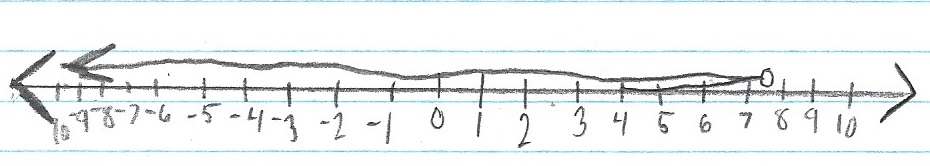
\includegraphics{ineq_1}

\begin{align*}
-5x + 9 &\geq 24 \\
-5x + {\cancel{9}} -{\cancel{9}} &\geq 24 - 9 \\
-5x &\geq 15 \\
\frac{\cancel{-5}x}{\cancel{-5}} &\leq \frac{15}{-5} \\
x &\leq -3
\end{align*}

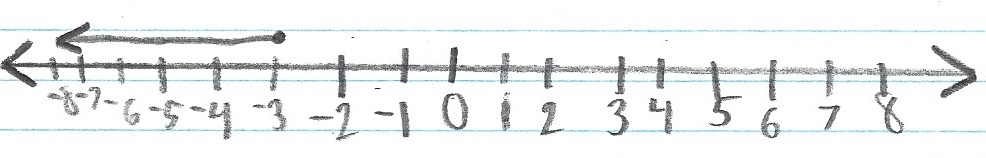
\includegraphics{ineq_2}

\begin{align*}
3x - 5 &\leq 2x - 13 \\
3x - {\cancel{5}} + {\cancel{5}} &\leq 2x - 13 + 5 \\
3x &\leq 2x - 8 \\
3x - 2x &\leq {\cancel{2x}} - {\cancel{2x}} - 8 \\
x &\leq -8
\end{align*}

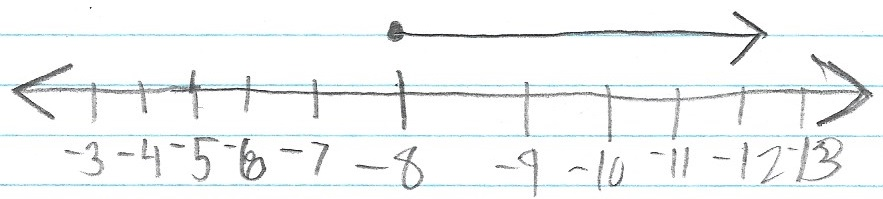
\includegraphics{ineq_3}

\section{Functions and Graphing}

Identify each ordered pair. Create a list of the domain and range.

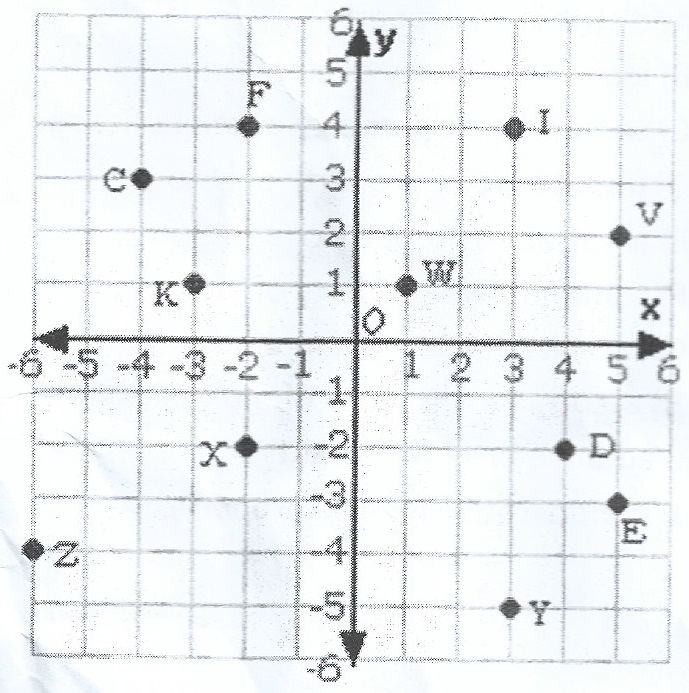
\includegraphics{graph_1}

I(3,4), V(5,2), W(1,1), F(-2,4), K(-3,1), C(-4,3), X(-2,-2), Z(-6,-4), Y(3,-5), D(4,-2), E(5,-3)

domain: \{-6, -4, -3, -2, 1, 3, 4, 5\}

range: \{-5, -4, -3, -2, 1, 2, 3, 4\}

\section{Label the Following Items on the Coordinate Plane}

\begin{itemize}
\item $x$-axis
\item $y$-axis
\item quadrant I
\item quadrant II
\item quadrant III
\item quadrant IV
\item origin
\end{itemize}
Plot the following points on the coordinate plane: \\
(1, 3), (-2, 4), (0, -1), (4, -5), (-3, 0), (-3, -2) \\

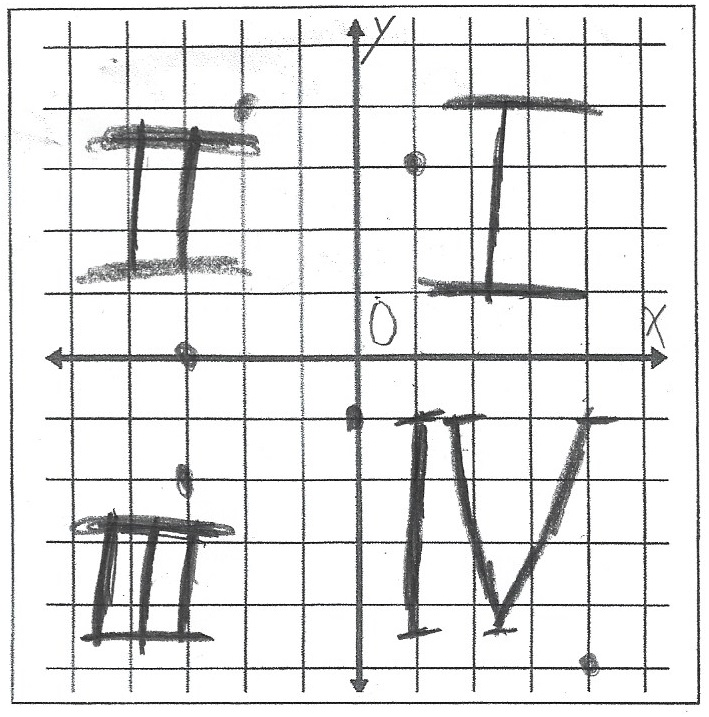
\includegraphics{graph_2}

\section{Properties}

Match each property to the appropriate description. Write your answer in the space provided. \\

\begin{tabular}{| c | l | l |}
\hline
G & $ 5 \times 1 = 5$  &  A) distributive property \\
H & $(22 \times 1) \times 9 = 22 \times (1 \times 9)$ & B) identity property of addition \\
B & $6 + 0 = 6$ & C) commutative property of multiplication \\
F & $3 + 4 = 4 + 3$ & D) multiplicative property of zero \\
A & $3(6 + 7) = (3 \times 6) + (3 \times 7)$ & E) associative property of addition \\
C & $4 \times 9 = 9 \times 4$ & F) commutative property of addition \\
E & $7 + (5 + 6) = (7 + 5) + 6$ & G) identity property of multiplication \\
J & $4/5 \times 5/4 = 20/20 = 1$ & H) associative property of multiplication \\
I & $5 + (-5) = 0$ & I) additive inverse property \\
D & $8 \times 0 = 0$ & J) multiplicative inverse property \\
\hline
\end{tabular}

\section{Circle All that Are a Rational Number}

\tikz \node[circle,draw]{$\sqrt{100}$};
\\
\tikz \node[circle,draw]{$\sqrt{36}$};
\\
$\sqrt{50}$
\\
$\sqrt{27}$
\\
\tikz \node[circle,draw]{$\sqrt{16}$};

\section{Define a perfect square}

A perfect square is an integer multiplied by itself.

\section{Explain what would be different to solve a cube root}



\end{document}
